\documentclass[12pt,a4paper]{report}

\usepackage[spanish]{babel}
\usepackage[T1]{fontenc}
\usepackage[utf8]{inputenc}
\usepackage{amsmath}
\usepackage{graphicx}
\usepackage[page]{appendix}
\usepackage{listings}
\usepackage{color}
\usepackage{float}
\usepackage{rotating}
\usepackage{graphicx}
\newcommand\scalemath[2]{\scalebox{#1}{\mbox{\ensuremath{\displaystyle #2}}}}

\addto\captionsspanish{\renewcommand\appendixpagename{Archivos de código}}

\DeclareFixedFont{\ttb}{T1}{txtt}{bx}{n}{9}
\DeclareFixedFont{\ttm}{T1}{txtt}{m}{n}{9} 
\DeclareFixedFont{\tti}{T1}{txtt}{m}{it}{9}
\definecolor{comment}{RGB}{150,150,150}

\lstset{
	frame = single, 
	extendedchars=true,	
	showstringspaces=false,
	inputencoding=latin1,
	literate={á}{{\'a}}1 {é}{{\'e}}1 {í}{{\'i}}1 {ó}{{\'o}}1 {ú}{{\'u}}1 {ñ}{{\~n}}1
	{Á}{{\'A}}1 {É}{{\'E}}1 {Í}{{\'I}}1 {Ó}{{\'O}}1 {Ú}{{\'U}}1,
	language=Python,
	basicstyle=\ttm,
	otherkeywords={self},
	keywordstyle=\ttb,
	commentstyle=\tti\color{comment}
	}




% Indica el título del documento como la palabra "Práctica " seguida del número de práctica.
\title{Práctica 1}

% Indica tu nombre completo
\author{Antonio Jesús Heredia Castillo}

\begin{document}

\maketitle

\section*{Ejercicio 1}
Represente las posiciones de los puntos respecto de la trama $\{A\}$ cuando:
\begin{enumerate}
	\item La trama $\{B\}$ se gira un ángulo $\alpha=90º$ alrededor del eje $X_A$
	\item La trama $\{B\}$ se gira un ángulo $\alpha=90º$ alrededor del eje $Y_A$
	\item La trama $\{B\}$ se gira un ángulo $\alpha=90º$ alrededor del eje $Z_A$
\end{enumerate}
Al comienzo las tramas $A$ y $B$ están superpuestas.En las siguientes graficas podremos ver la trama $A$ en color azul y la trama $B$ girada de color naranja. El resultado de girar $\{B\}$ un ángulo $\alpha=90º$ alrededor del eje $X_A$ lo podemos ver en la Figura \ref{fig:eje1_a}.
\begin{figure}[H]
	\centering
	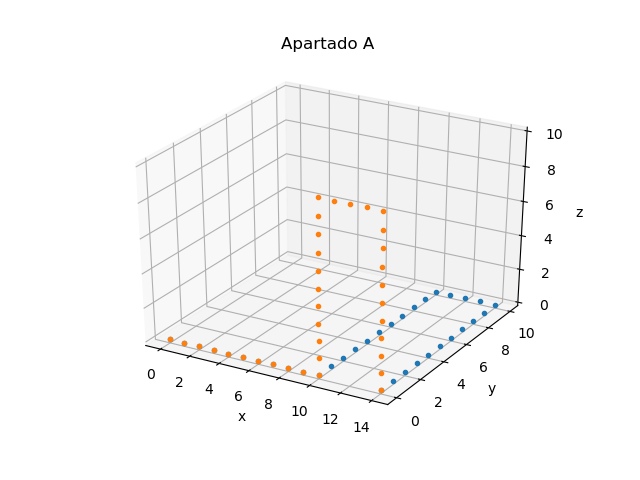
\includegraphics[width=0.7\linewidth]{img/eje1_a.png}
	\caption{Rotación de $90º$ en $X_A$}
	\label{fig:eje1_a}
\end{figure}
Para realizar la rotación anterior he usado la siguiente matriz de rotación:
$$
\begin{pmatrix}
		1 & 0 & 0 \\ 
		0 & cos(90) & -sin(90) \\ 
		0 & sin(90) & cos(90) 
\end{pmatrix}
$$
El resultado de girar $\{B\}$ un ángulo $\alpha=90º$ alrededor del eje $Y_A$ lo podemos ver en la Figura \ref{fig:eje1_b}.
\begin{figure}[H]
	\centering
	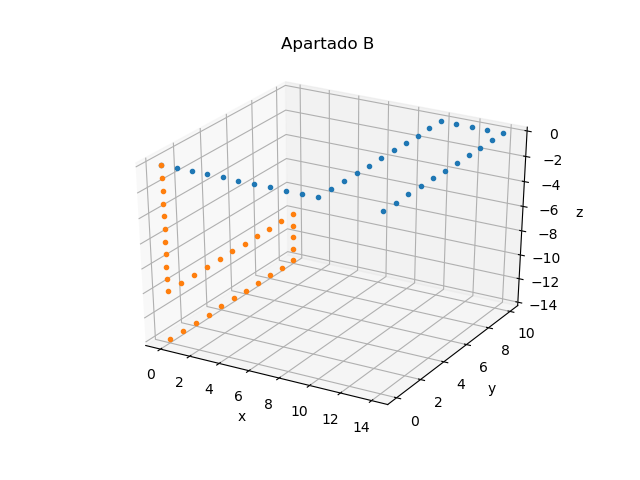
\includegraphics[width=0.7\linewidth]{img/eje1_b.png}
	\caption{Rotación de $90º$ en $Y_A$}
	\label{fig:eje1_b}
\end{figure}
Para realizar la rotación anterior he usado la siguiente matriz de rotación:
$$
\begin{pmatrix} 
		cos(90) & 0 & sin(90) \\  
		0 & 1 & 0 \\  
		-sin(90)& 0 & cos(90) \\  
\end{pmatrix}
$$
El resultado de girar $\{B\}$ un ángulo $\alpha=90º$ alrededor del eje $Z_A$ lo podemos ver en la Figura \ref{fig:eje1_c}.
\begin{figure}[H]
	\centering
	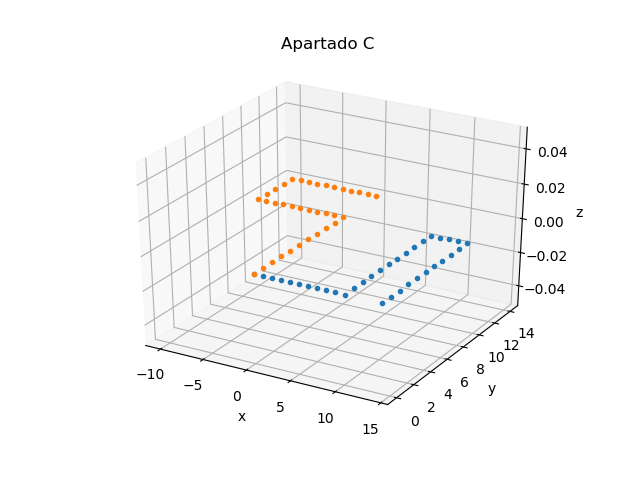
\includegraphics[width=0.7\linewidth]{img/eje1_c.png}
	\caption{Rotación de $90º$ en $Z_A$}
	\label{fig:eje1_c}
\end{figure}
Para realizar la rotación anterior he usado la siguiente matriz de rotación:
$$
\begin{pmatrix} 
		cos(90) & -sin(90) & 0 \\  
		sin(90) & cos(90) & 0 \\  
		0& 0 & 1 \\  
\end{pmatrix}
$$

Usando simplemente las matriz de rotación podemos conseguir la rotación de todos los puntos respecto a un eje. El único punto que no cambia es el situado en el $\{0,0,0\}$ que sea la que sea la matriz de rotación que se le aplique no cambia su posición.
\section*{Ejercicio 2}
Represente las posiciones de los puntos respecto de la trama $\{A\}$ cuando la
trama $\{B\}$ del ejercicio anterior se rota desde la posición original (superpuesta
a la trama $\{A\}$) en torno al eje $X_B$ un ángulo $\gamma = 60º$, a continuación se gira
en torno al eje $Y_B$ un ángulo $\beta = 90º$, y después se gira en torno al eje $Z_B$ un
ángulo $\alpha= 30º$.\\\\
Lo primero que voy a hacer es indicar las matrices que voy a usar en este ejercicio aunque son las mismas que en el ejercicio anterior pero cambiando los ángulos. La rotación en X sera la siguiente:
$$
\begin{pmatrix}
1 & 0 & 0 \\ 
0 & cos(60) & -sin(60) \\ 
0 & sin(60) & cos(60) 
\end{pmatrix}
$$
La rotación en Y sera:
$$
\begin{pmatrix} 
cos(90) & 0 & sin(90) \\  
0 & 1 & 0 \\  
-sin(90)& 0 & cos(90) \\  
\end{pmatrix}
$$
Por ultimo la rotación en Z sera:
$$
\begin{pmatrix} 
cos(30) & -sin(30) & 0 \\  
sin(30) & cos(30) & 0 \\  
0& 0 & 1 \\  
\end{pmatrix}
$$
Vamos a ver que ocurre si realizamos las rotaciones en el orden que nos dice el enunciado.\\
Primero realizamos la rotación de $60º$ en el eje $X_B$ como se puede ver en la Figura \ref{fig:eje2a_x}.
\begin{figure}[H]
	\centering
	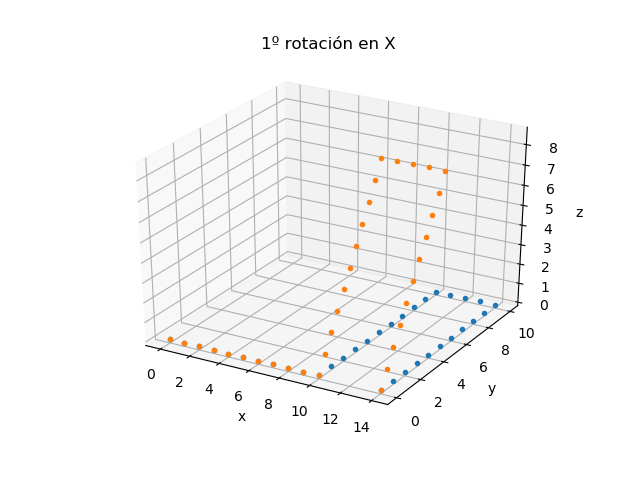
\includegraphics[width=0.7\linewidth]{img/eje2a_x.png}
	\caption{Rotación de $60º$ en $X_B$}
	\label{fig:eje2a_x}
\end{figure}
A continuación realizamos la rotación de $90º$ en el eje $Y_B$ y obtendremos lo que vemos en la Figura \ref{fig:eje2a_y}.
\begin{figure}[H]
	\centering
	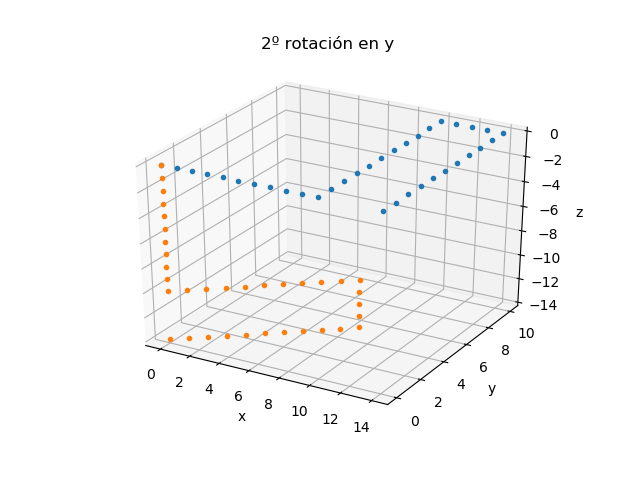
\includegraphics[width=0.7\linewidth]{img/eje2a_y.png}
	\caption{Rotación de $90º$ en $Y_B$}
	\label{fig:eje2a_y}
\end{figure}
Por ultimo realizamos la rotación de $30º$ en el eje $Z_B$ quedando la Figura \ref{fig:eje2a_x}.
\begin{figure}[H]
	\centering
	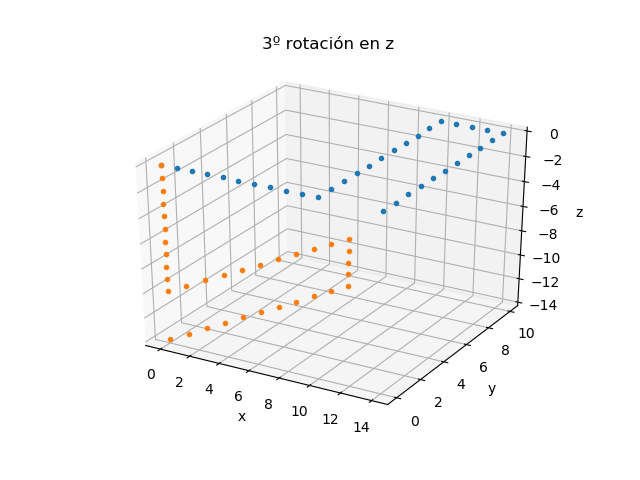
\includegraphics[width=0.7\linewidth]{img/eje2a_z.png}
	\caption{Rotación de $30º$ en $Z_B$}
	\label{fig:eje2a_z}
\end{figure}

Estas rotaciones se pueden ver mejor cuando obtenemos la grafica desde python, ya que podemos mover los ejes y cambiar la vista para tener una mejor perspectiva de la posición. Ya que de la Figura \ref{fig:eje2a_y} a la Figura \ref{fig:eje2a_z} parece a primera vista que no cambia mucho, pero si que se nota el cambio. \\ \\Ahora vamos a ver que ocurre si realizamos las mismas rotaciones con los mismo grados pero en diferente orden.
Primero realizamos la rotación de $60º$ en el eje $X_B$ como se puede ver en la Figura \ref{fig:eje2b_y}.
\begin{figure}[H]
	\centering
	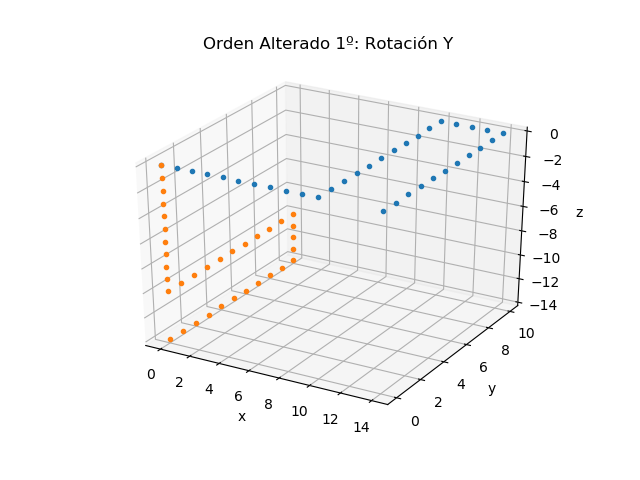
\includegraphics[width=0.7\linewidth]{img/eje2b_x.png}
	\caption{Rotación de $90º$ en $Y_B$}
	\label{fig:eje2b_y}
\end{figure}
A continuación realizamos la rotación de $30º$ en el eje $Z_B$ y obtendremos lo que vemos en la Figura \ref{fig:eje2b_z}.
\begin{figure}[H]
	\centering
	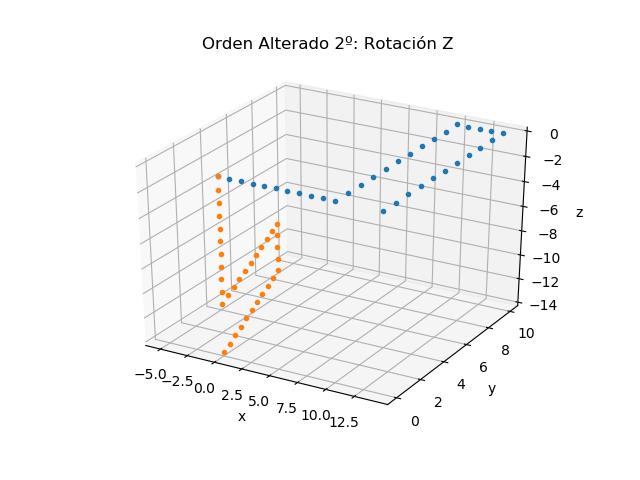
\includegraphics[width=0.7\linewidth]{img/eje2b_y.png}
	\caption{Rotación de $90º$ en $Z_B$}
	\label{fig:eje2b_z}
\end{figure}
Por ultimo realizamos la rotación de $60º$ en el eje $X_B$ quedando la Figura \ref{fig:eje2b_x}.
\begin{figure}[H]
	\centering
	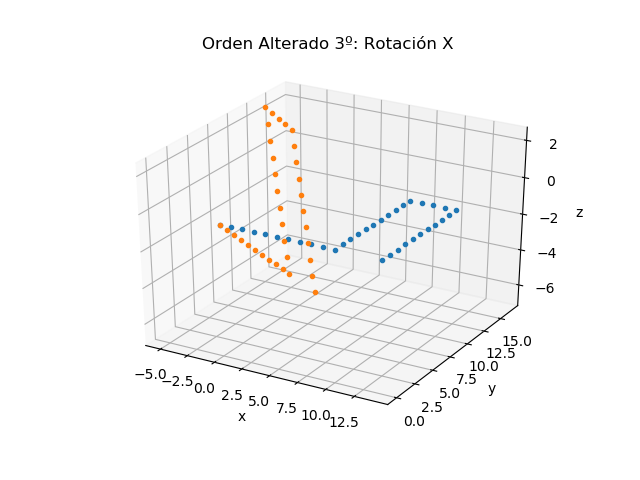
\includegraphics[width=0.7\linewidth]{img/eje2b_z.png}
	\caption{Rotación de $30º$ en $X_B$}
	\label{fig:eje2b_x}
\end{figure}

Comparando la Figura \ref{fig:eje2a_z} (realizando en el orden adecuado las rotaciones) y la Figura \ref{fig:eje2b_x} (en un orden distinto al dado), podemos ver que no obtenemos la misma posición final a pesar de haber ejecutado las mismas rotaciones (se puede observar en el código que son las mismas matrices de rotación).
\section*{Ejercicio 3}
Diseñe e implemente una función en Python que reciba como entrada un numpy array de dimensión $n \times 4$ con los parámetros de Denavit-Hartenberg de un
manipulador cualquiera, y devuelva como salida la matriz de transformación
homogénea (como un numpy array de dimensión $4 \times 4$) que relaciona el sistema
de coordenadas del efector y el sistema de coordenadas de la base. Contemple la posibilidad de que los ángulos de rotación y los desplazamientos sean variables
simbólicas (use el paquete sympy). Compruebe el correcto funcionamiento de
 la función con algunos ejemplos.\\\\
Para implementar la función he usado un "bucle for" que recorra las diferentes filas de la matriz de entrada y para cada una de las cuatros variables genere su matriz de rotación o de traslación correspondiente. Una vez obtenidas las matrices que llamare $rz$, $dz$, $dx$ y $rx$ las multiplicara para obtener la matriz $^{i}T_{i+1}$ que multiplicada por la matriz homogénea anterior nos dará  $^{0}T_{i+1}$. En el primer paso del "bucle for" la matriz homogénea sera la matriz identidad. Cuando termina el "bucle for" ya tenemos la matriz homogénea para pasar desde $0$ hasta $n$. Esto se puede ver de forma mas clara en el código que se adjunta.\\\\
Una vez implementada la función, pase a comprobar que funcionaba usando el mismo ejemplo de las transparencias de clase, para tener un ejemplo que se que era correcto.
Teniendo una entrada como la siguiente:
$$\begin{matrix}
\hline q & \theta_{i} & d_{i} & a_{i} & \alpha_{i}  \\
\hline 1 & q_{1} & l_{1} & 0 & 0 \\
2 & 90^{\circ} & q_{2} & 0 & 90^{\circ} \\
3 & 0 & l_{3}+q_{3} & 0 & 0
\end{matrix}
$$

Debemos obtener (y obtenemos) el siguiente resultado:
$$
\begin{pmatrix}
-sin(q_1) & 0 & cos(q_1)&(l_3+q_3)*cos(q_1) \\
cos(q_1) & 0 & sin(q_1)&(l_3+q_3)*sin(q_1) \\
0 & 1 & 0&(l_1+q_2) \\
0 & 0 & 0&1 \\
\end{pmatrix}
$$
Podemos ver el resultado de la ejecución en la Figura \ref{fig:ej31}
\begin{figure}[H]
	\centering
	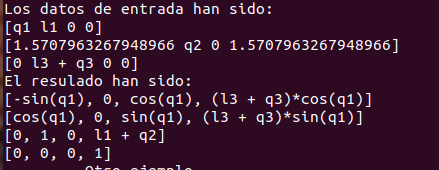
\includegraphics{img/ej3_1}
	\caption{Resultado de la función usando los datos de ejemplo}
	\label{fig:ej31}
\end{figure}

También lo he comprobado usando los datos del ``Ejercicio 1'' de la relación de ejercicios 3. Los datos de entrada serán:
$$
\begin{matrix}
\hline q & \theta_{i} & d_{i} & a_{i} & \alpha_{i}  \\
\hline 1 & q_{1} & 0 & l_{1} & 0 \\
2 & q_2 & 0 & l_{2} & 0 \\
\end{matrix}
$$
Y debemos de obtener como resultado:
\\\\
\scalemath{0.5}{$$\begin{pmatrix}
cos(q_1)*cos(q_2)-sin(q_1)*sin(q_2) & -sin(q1)*cos(q2) - sin(q2)*cos(q1) & 0 &l1*cos(q1) - l2*sin(q1)*sin(q2) + l2*cos(q1)*cos(q2) \\
sin(q1)*cos(q2)+ sin(q2)*cos(q1) & -sin(q1)*sin(q2) + cos(q1)*cos(q2) & 0 &	l1*sin(q1) + l2*sin(q1)*cos(q2) + l2*sin(q2)*cos(q1) \\
0 & 0 & 1&0 \\
0 & 0 & 0&1 \\
\end{pmatrix}$$}\\\\
Que es justo lo que obtenemos como podemos ver en la Figura \ref{fig:ej32}.
\begin{figure}[H]
	\centering
	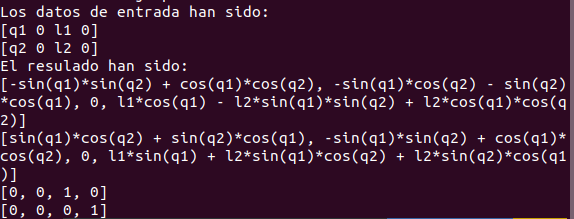
\includegraphics{img/ej3_2}
	\caption{Resultado de la función usando los datos del ejercicio 1}
	\label{fig:ej32}
\end{figure}Los resultados se pueden comprobar ejecutando el programa "Denavit\_Hatenberg.py".
\begin{appendices}
	\section*{ejercicio1.py}
	\lstinputlisting{../ejercicio1.py}
	\section*{ejercicio2.py}
	\lstinputlisting{../ejercicio2.py}
	\section*{Denavit\_Hartenberg.py}
	\lstinputlisting{../Denavit_Hartenberg.py}
\end{appendices}

\end{document}
